\documentclass[a4paper,11pt]{exam}
\printanswers % pour imprimer les réponses (corrigé)
%\noprintanswers % Pour ne pas imprimer les réponses (énoncé)
\addpoints % Pour compter les points
% \noaddpoints % pour ne pas compter les points
%\qformat{\textbf{\thequestion ) } }
%\qformat{\textbf{\thequestion )}} % Pour définir le style des questions (facultatif)
\usepackage{color} % définit une nouvelle couleur
\shadedsolutions % définit le style des réponses
% \framedsolutions % définit le style des réponses
\definecolor{SolutionColor}{rgb}{0.8,0.9,1} % bleu ciel
\renewcommand{\solutiontitle}{\noindent\textbf{Solution:}\par\noindent} % Définit le titre des solutions




\makeatletter

\def\maketitle{{\centering%
	\par{\huge\textbf{\@title}}%
	\par{\@date}%
	\par}}


\renewcommand{\thesubsection}{\Alph{subsection}.}   

\makeatother

\lhead{NOM Pr\'enom :}
\rhead{\textbf{Les r\'eponses doivent \^etre justifi\'ees et r\'edig\'ees}}
\cfoot{\thepage / \pageref{LastPage}}


%\usepackage{../../pas-math}
%\usepackage{../../moncours}


%\usepackage{pas-cours}
%-------------------------------------------------------------------------------
%          -Packages nécessaires pour écrire en Français et en UTF8-
%-------------------------------------------------------------------------------
\usepackage[utf8]{inputenc}
\usepackage[frenchb]{babel}
%\usepackage{numprint}
\usepackage[T1]{fontenc}
%\usepackage{lmodern}
\usepackage{textcomp}
\usepackage[french, boxed]{algorithm2e}
\usepackage{hyperref}


%-------------------------------------------------------------------------------

%-------------------------------------------------------------------------------
%                          -Outils de mise en forme-
%-------------------------------------------------------------------------------
\usepackage{hyperref}
\hypersetup{pdfstartview=XYZ}
%\usepackage{enumerate}
\usepackage{graphicx}
\usepackage{multicol}
\usepackage{tabularx}
\usepackage{multirow}
\usepackage{color}
\usepackage{eurosym}


\usepackage{anysize} %%pour pouvoir mettre les marges qu'on veut
%\marginsize{2.5cm}{2.5cm}{2.5cm}{2.5cm}

\usepackage{indentfirst} %%pour que les premier paragraphes soient aussi indentés
\usepackage{verbatim}
\usepackage{enumitem}
\usepackage{booktabs}
\usepackage[usenames,dvipsnames,svgnames,table]{xcolor}

\usepackage{variations}

%-------------------------------------------------------------------------------


%-------------------------------------------------------------------------------
%                  -Nécessaires pour écrire des mathématiques-
%-------------------------------------------------------------------------------
\usepackage{amsfonts}
\usepackage{amssymb}
\usepackage{amsmath}
\usepackage{amsthm}
\usepackage{tikz}
\usepackage{xlop}
\usepackage[output-decimal-marker={,}]{siunitx}
%-------------------------------------------------------------------------------

%-------------------------------------------------------------------------------
%                  -Nécessaires pour écrire des formules chimiquess-
%-------------------------------------------------------------------------------

\usepackage[version=4]{mhchem}

%-------------------------------------------------------------------------------
% Pour pouvoir exploiter les fichiers directement dans beamer
\newcommand{\pause}{\ }
%-------------------------------------------------------------------------------
%                    - Mise en forme avancée
%-------------------------------------------------------------------------------

\usepackage{ifthen}
\usepackage{ifmtarg}


\newcommand{\ifTrue}[2]{\ifthenelse{\equal{#1}{true}}{#2}{$\qquad \qquad$}}

%\newcommand{\kword}[1]{\textcolor{red}{\underline{#1}}}
%-------------------------------------------------------------------------------

%-------------------------------------------------------------------------------
%                     -Mise en forme d'exercices-
%-------------------------------------------------------------------------------
%\newtheoremstyle{exostyle}
%{\topsep}% espace avant
%{\topsep}% espace apres
%{}% Police utilisee par le style de thm
%{}% Indentation (vide = aucune, \parindent = indentation paragraphe)
%{\bfseries}% Police du titre de thm
%{.}% Signe de ponctuation apres le titre du thm
%{ }% Espace apres le titre du thm (\newline = linebreak)
%{\thmname{#1}\thmnumber{ #2}\thmnote{. \normalfont{\textit{#3}}}}% composants du titre du thm : \thmname = nom du thm, \thmnumber = numéro du thm, \thmnote = sous-titre du thm

%\theoremstyle{exostyle}
%\newtheorem{exercice}{Exercice}
%
%\newenvironment{questions}{
%\begin{enumerate}[\hspace{12pt}\bfseries\itshape a.]}{\end{enumerate}
%} %mettre un 1 à la place du a si on veut des numéros au lieu de lettres pour les questions 
%-------------------------------------------------------------------------------

%-------------------------------------------------------------------------------
%                    - Mise en forme de tableaux -
%-------------------------------------------------------------------------------

\renewcommand{\arraystretch}{1.7}

\setlength{\tabcolsep}{1.2cm}

%-------------------------------------------------------------------------------



%-------------------------------------------------------------------------------
%                    - Racourcis d'écriture -
%-------------------------------------------------------------------------------
%Droites
\newcommand{\dte}[1]{$(#1)$}
\newcommand{\fig}[1]{figure $#1$}
\newcommand{\sym}{symétrique}
\newcommand{\syms}{symétriques}
\newcommand{\asym}{axe de symétrie}
\newcommand{\asyms}{axes de symétrie}
\newcommand{\seg}[1]{$[#1]$}
\newcommand{\monAngle}[1]{$\widehat{#1}$}
\newcommand{\bissec}{bissectrice}
\newcommand{\mediat}{médiatrice}
\newcommand{\ddte}[1]{$[#1)$}


% Angles orientés (couples de vecteurs)
\newcommand{\aopp}[2]{(\vec{#1}, \vec{#2})} %Les deuc vecteurs sont positifs
\newcommand{\aopn}[2]{(\vec{#1}, -\vec{#2})} %Le second vecteur est négatif
\newcommand{\aonp}[2]{(-\vec{#1}, \vec{#2})} %Le premier vecteur est négatif
\newcommand{\aonn}[2]{(-\vec{#1}, -\vec{#2})} %Les deux vecteurs sont négatifs

%Ensembles mathématiques
\newcommand{\naturels}{\mathbb{N}} %Nombres naturels
\newcommand{\relatifs}{\mathbb{Z}} %Nombres relatifs
\newcommand{\rationnels}{\mathbb{Q}} %Nombres rationnels
\newcommand{\reels}{\mathbb{R}} %Nombres réels
\newcommand{\complexes}{\mathbb{C}} %Nombres complexes


%Intégration des parenthèses aux cosinus
\newcommand{\cosP}[1]{\cos\left(#1\right)}
\newcommand{\sinP}[1]{\sin\left(#1\right)}


%Probas stats
\newcommand{\stat}{statistique}
\newcommand{\stats}{statistiques}


\newcommand{\homo}{homothétie}
\newcommand{\homos}{homothéties}


\newcommand{\mycoord}[3]{(\textcolor{red}{\num{#1}} ; \textcolor{Green}{\num{#2}} ; \textcolor{blue}{\num{#3}})}
%-------------------------------------------------------------------------------

%-------------------------------------------------------------------------------
%                    - Mise en page -
%-------------------------------------------------------------------------------

\newcommand{\twoCol}[1]{\begin{multicols}{2}#1\end{multicols}}


\setenumerate[1]{font=\bfseries,label=\textit{\alph*})}
\setenumerate[2]{font=\bfseries,label=\arabic*)}


%-------------------------------------------------------------------------------
%                    - Elements cours -
%-------------------------------------------------------------------------------

%Correction d'exercice
\newcommand{\exoSec}[2]{\subsection*{Exercice #1 page #2}}
%-------------------------------------------------------------------------------
%                    - raccourcis d'écriture -
%-------------------------------------------------------------------------------

%Mise en évidence de termes clés
\newcommand{\mykw}[1]{\textcolor{red}{\underline{\textbf{#1}}}}

%Exercices
\newcommand{\exo}[2]{exercice #1 page #2}
\newcommand{\Exo}[2]{Exercice #1 page #2}

\renewcommand{\pause}{\ }

%Intervalles
\newcommand{\interOO}[2]{$]$#1 , #2$[$}
\newcommand{\interOF}[2]{$]$#1 , #2$]$}
\newcommand{\interFO}[2]{$[$#1 , #2$[$}
\newcommand{\interFF}[2]{$[$#1 , #2$]$}



%\usepackage{fullpage}
\author{\ }
\date{15 Mars 2018}
\title{Sciences Physiques : DS n° 3}


\begin{document}
%	\usepackage{fancyhdr}
%	
%	\pagestyle{fancy}
%	\fancyhf{}
	%\rhead{Share\LaTeX}

	\maketitle
	
\begin{small}
	\begin{center}
		\begin{tabular}{|@{\ }l@{}|@{\ }c@{\ }|}
			\hline
			\textbf{Compétence} & \textbf{Maitrise} \\
			\hline
		Notions de molécules, atomes, ions. \ \ &  \ \ \ \\
			\hline
			Conservation de la masse lors d’une transformation chimique. &  \\
			\hline			
			Associer leurs symboles aux éléments à l’aide de la classification périodique. \ &  \\
			\hline
			Interpréter une formule chimique en termes atomiques. &  \\
			\hline
		\end{tabular}
	\end{center}
\end{small}	
	
	
\vspace*{-0.5cm}	

%\section{\'Equations de réaction}

Ajuster les équations de réactions suivantes :
\begin{questions}
	\question $CH_4 + ....O_2 \rightarrow ....CO_2 + ....H_2O$
	
	\question $C_7H_{16} + ....O_2 \rightarrow ....CO_2 + ....H_2O$	
	
	\question $C_6H_{2}O + ....O_2 \rightarrow ....CO_2 + ....H_2O$
\end{questions}


%\section{À chaque modèle sa formule}
\begin{questions}
	\question \'A partir de ces dessins de modèles, donner la formule des molécules suivantes.

	\begin{center}
		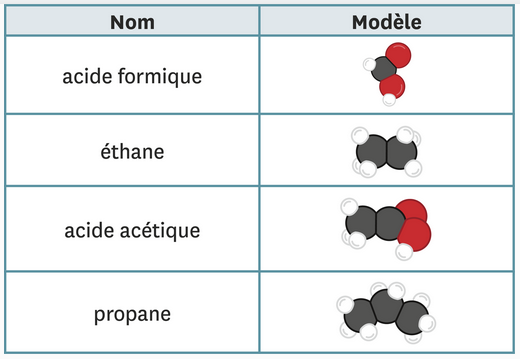
\includegraphics[scale=0.6]{img/exemples}
	\end{center}
	\fillwithdottedlines{2cm}
	
\end{questions}

\section{Composition des molécules}


\begin{questions}
	\question Donner la composition des molécules suivantes :
	
	\begin{parts}
		\part l'éthylène $C_2H_4$	
		\fillwithdottedlines{1cm}
		
		\part le monoxyde d'azote $NO$	
		\fillwithdottedlines{1cm}
		
		\part l'ozone $O_3$	
		\fillwithdottedlines{1cm}	
		
		\part l'eau oxygénée $H_2O_2$	
		\fillwithdottedlines{1cm}
	\end{parts}

\end{questions}


%\newpage





\section{Phrases à compléter (3 points)}

Recopier et compléter les phrases suivantes :

\begin{questions}
	\question[\half] Dans un circuit, plus la résistance augmente, plus l'intensité du courant $....$ .
	\begin{solution}
		Dans un circuit, plus la résistance augmente, plus l'intensité du courant \textbf{diminue}.
	\end{solution}
	
	\question[1] La résistance électrique se mesure à l'aide d'un $....$ et s'exprime en $....$ .
	\begin{solution}
		La résistance électrique se mesure à l'aide d'un \textbf{ohmmètre} et s'exprime en \textbf{ohm} .
	\end{solution}
	
	\question[1\half] La tension aux bornes d'un conducteur ohmique est $....$ à l'intensité du courant qui le traverse : c'est la loi d'Ohm, que l'on traduit par la relation : $....$ = $R$ $\times$  $....$.
	
	\begin{solution}
		La tension aux bornes d'un conducteur ohmique est \textbf{proportionnelle} à l'intensité du courant qui le traverse : c'est la loi d'Ohm, que l'on traduit par la relation : $\mathbf{U}$ = $R$ $\times$  $\mathbf{I}$.
	\end{solution}
\end{questions}



\newpage


\section{La corrosion du fer (5 points)}

Au contact du dioxygène $O_2$ et en présence d'eau $H_2O$, le fer $Fe$ se corrode en rouille $Fe_2O_3$. L'eau est indispensable pour ce processus, mais lors de cette transformation la quantité totale d'eau reste la même. On propose une équation pour modéliser cette réaction : 

\begin{center}
	\ce{4Fe + 4O2 -> 2Fe2O3}
\end{center}
%\begin{equation}
%	4 Fe + 4 O_2 \rightarrow 2 Fe_2O_3
%\end{equation}


\begin{questions}
	\question[1] Expliquer pourquoi l'eau n'est ni un réactif, ni un produit dans cette transformation.
	\fillwithdottedlines{2cm}
	\begin{solution}
		Le texte indique que dans cette réaction, la quantité d'eau ne change pas donc il n'est pas nécessaire de la faire apparaître dans l'équation de réaction.
	\end{solution}
	
	\question[1] Compter le nombre d'atomes de fer dans les réactifs puis dans les produits de l'équation.
	\fillwithdottedlines{2cm}
	\begin{solution}
		Dans les réactifs il y a 4 atomes de fer et dans les produits il y en 4 aussi.
	\end{solution}
	
	\question[1] Faire de même pour les atomes d'oxygène.
	\fillwithdottedlines{2cm}
	\begin{solution}
		Dans les réactifs il y a 8 atomes d'oxygène et dans les produits il y en a 6.
	\end{solution}
	
	\question[2] Indiquer à l'aide des réponses précédentes, si l'équation de réaction est équilibrée. Si ce n'est pas le cas, proposer une correction de l'équation.
	\fillwithdottedlines{3cm}
	\begin{solution}
		Il n'y a pas le même nombre d'atomes d'oxygène dans les réactifs et les produits donc l'équation de réaction n'est pas équilibrée. 
		
		Dans l'équation suivante il y a autant d'atomes de fer et d'oxygène dans les réactifs que dans les produits, elle est donc équilibrée :
		\begin{center}
			\ce{4Fe + 3O2 -> 2Fe2O3}
		\end{center}
	\end{solution}
\end{questions}


%\newpage

\section{Structure des atomes}\label{ex:structure}

\begin{questions}
	\question[4] Compléter le tableau \\
	
	\noindent\begin{tabular}{|@{\ }l@{\ }|@{\ }c@{\ }|@{\ }c@{\ }|@{\ }c@{\ }|@{\ }c@{\ }|@{\ }c@{\ }|}
			\hline
		\textbf{Nom de l'atome}                  &  $\qquad\quad\qquad$     & Chlore &  $\qquad\quad\qquad$  &  $\qquad\:\qquad$  & $\qquad\quad\qquad$    \\ \hline
		\textbf{Symbole de l'atome}              & $He$ &        &    &    & $H$ \\ \hline
		\textbf{Nombre de protons dans le noyau} &      &        & 26 &    &     \\ \hline
		\textbf{Nombre d'électrons}              &      &        &    & 79 &    \\ \hline
	\end{tabular}

%	\begin{solution}
%		\noindent\begin{tabular}{|@{\ }l@{\ }|@{\ }c@{\ }|@{\ }c@{\ }|@{\ }c@{\ }|@{\ }c@{\ }|@{\ }c@{\ }|}
%			\hline
%			\textbf{Nom de l'atome}                  &  Hélium     & Chlore &  Fer  & Or  & Hydrogène    \\ \hline
%			\textbf{Symbole de l'atome}              & $He$ &   $Cl$     & $Fe$   & $Au$   & $H$ \\ \hline
%			\textbf{Nombre de protons dans le noyau} &   2   &  17    & 26 &  79  &  1   \\ \hline
%			\textbf{Nombre d'électrons}              &   2   &  17    & 26 &  79  &  1   \\ \hline
%		\end{tabular}
%	\end{solution}
\end{questions}


\newpage 

\section{L'atome de Fer (4 points)}

\begin{multicols}{2}
	
	
	Le métal fer est un cristal, ce qui veut dire que ses atomes sont organisés selon une structure bien particulière appelée maille élémentaire. Sur l'Atomium à Bruxelles, chaque sphère de 18 m de diamètre représente un atome de fer agrandi 64 milliards de fois.
	
	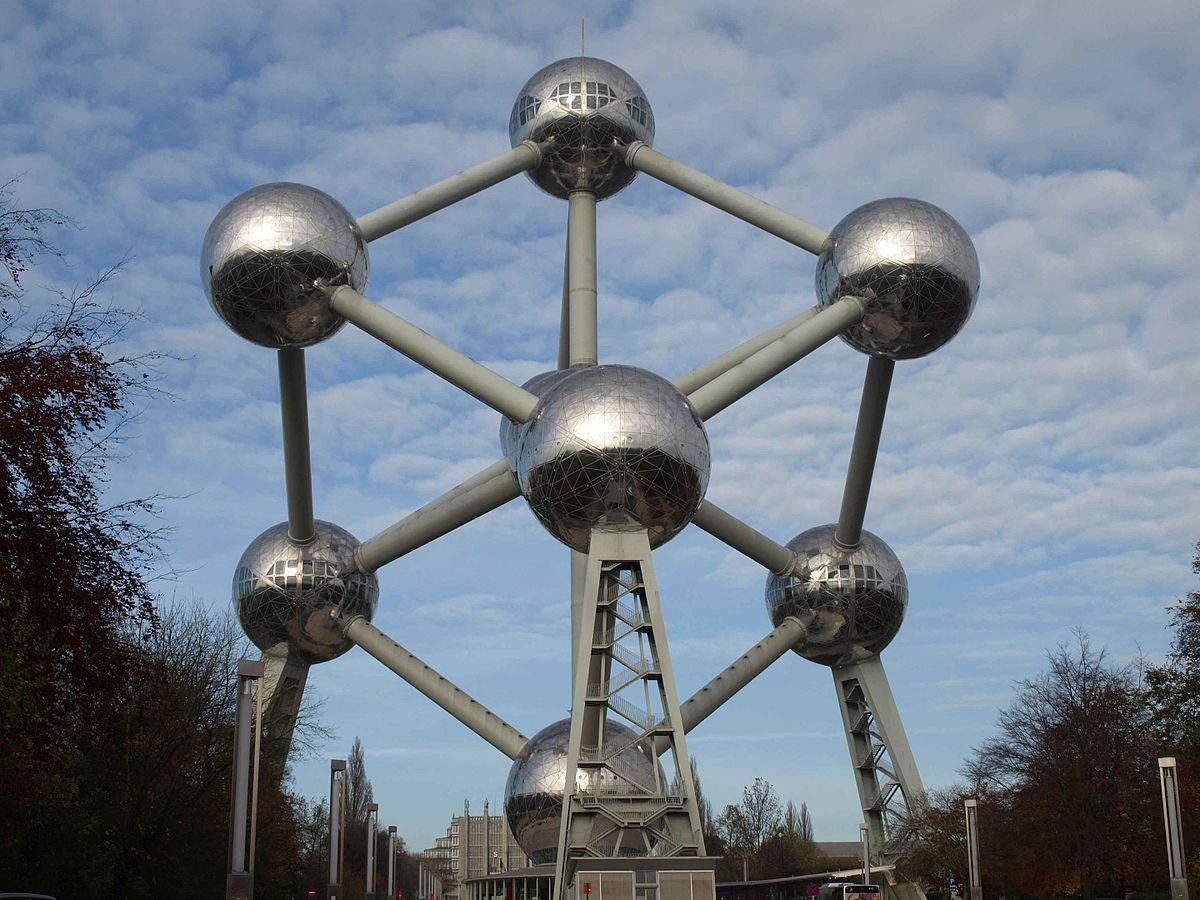
\includegraphics[scale=0.5]{img/atomium}
\end{multicols}


\begin{questions}
	\question[2] Calculer le diamètre d'un atome de fer.
	%\fillwithdottedlines{2cm}
	\begin{solution}
		64 milliards  = $64 \times 10^9$.
		\begin{eqnarray*}
			\dfrac{18}{64 \times 10^9}& = & \num{2.8125} \times 10^{-10} m \\
			& = & \num{281.25} \times 10^{-12} m \\
		\end{eqnarray*}
	Un atome de fer a un diamètre de $\num{281.25} pm$.
	\end{solution}
	  
	
	\question[1] Combien d'électrons contient-il ?
	%\fillwithdottedlines{2cm}
	\begin{solution}
		Le numéro atomique de l'atome de fer est 26, il contient 26 protons, et donc 26 électrons.
	\end{solution}
	
	\question[1] Quel est le diamètre du noyau d'un atome de fer ?
	%\fillwithdottedlines{3cm}
	\begin{solution}
		Le diamètre d'un atome est \num{100000} fois plus grand que celui de son noyau.
		
		\begin{eqnarray*}
			\dfrac{\num{2.8125} \times 10^{-10}}{10^5}& = & \num{2.8125} \times 10^{-15} m
		\end{eqnarray*}
	
	Donc le noyau d'un atome de fer a un diamètre de \num{2.8125} fm.
	\end{solution}
\end{questions}



\newpage 

\section{Représentation de la vitesse (6 points)}

\begin{questions}
	\question Représenter la vitesse d'un objet à un instant précis, dans les conditions suivantes  :
	
	\begin{parts}
		\part[2] \begin{itemize}
			\item Mouvement : horizontal de gauche à droite;
			\item Valeur de la vitesse : 25 m/s;
			\item \'Echelle choisie: 1 cm pour 10 m/s.
			
		\end{itemize}
	
		\makeemptybox{4cm}
		
		
		\part[2] \begin{itemize}
			\item Mouvement : chute verticale d'un objet;
			\item Valeur de la vitesse : 10 m/s;
			\item \'Echelle choisie: 1 cm pour 5 m/s.
			
		\end{itemize}
		
		\makeemptybox{4cm}
	\end{parts}

	\question[2] \'A l'aide d'un logiciel de traitement de vidéos, on peut repérer les positions successives prises par un point d'une grande roue lors de son mouvement.
	
	Sans tenir compte de la valeur de la vitesse, représenter la vitesse aux positions 3, 12, 22 et 33.
	
	\begin{center}
		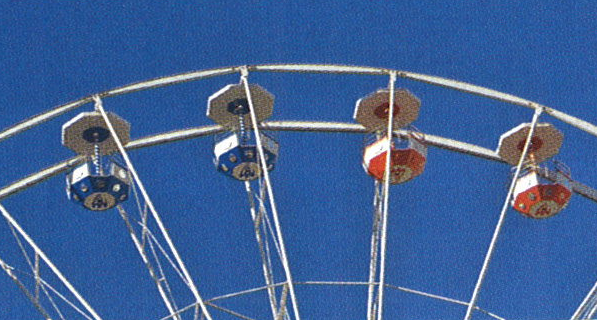
\includegraphics[scale=0.45]{roue}
	\end{center}
\end{questions}



 
%\newpage
%
%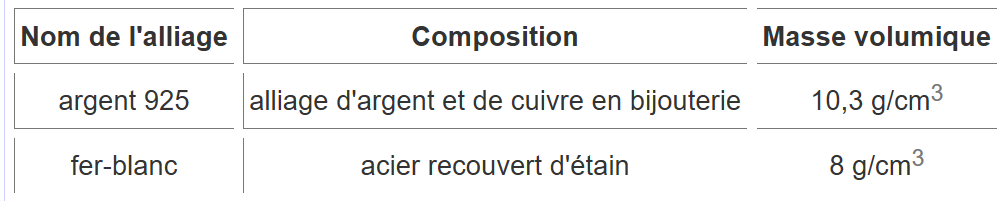
\includegraphics [scale=0.5, angle= 90 ]{img/tableau} 
\ \label{LastPage}

\end{document}